% Volume III: Probability, Statistics, Information, and Causality
% Continuity note for Chapter 15.
% Previous dependencies: Chapter 11's integration and change-of-variables discipline; Chapter 13's probability spaces, random variables, joint/marginal/conditional distributions, independence, random vectors, means, and covariance; Chapter 14's named distributions, likelihoods, multivariate Gaussians, and exponential-family parameters.
% New durable concepts: expectation as a weighted averaging operator; integrability; expectation of functions of random variables; linearity of expectation; variance as expected squared deviation; conditional expectation given an event, a value, and an observed variable; conditional expectation as a random variable and as best mean-square prediction; tower property; Bayes' theorem as reweighting hypotheses by likelihoods; evidence/normalization; conditional independence and likelihood factorization; actions, states, loss functions, posterior risk, Bayes actions, MAP decisions, posterior means, and asymmetric costs.
% Forward hooks: Chapter 16 uses expectation, variance, and conditional expectation to state LLN, CLT, convergence, and concentration; Chapter 17 turns Bayes rules, losses, and posterior risks into estimation, testing, model selection, and predictive risk; Chapter 18 reuses expectation inside entropy, KL divergence, cross-entropy, mutual information, and Fisher information; later filtering, graphical models, predictive coding, and neural decision chapters reuse conditioning, conditional independence, and Bayes actions.
% Notation commitments: Random variables are X,Y,Z; observed values are x,y,z; hypotheses or states are theta in Theta; actions are a in A; events are A,B with P(B)>0 when conditioning on B; distributions use p(x), p(x,y), p(x|y), p(theta), p(x|theta), and p(theta|x); expectation is \mathbb{E}[X], conditional expectation is \mathbb{E}[X|Y] or \mathbb{E}[X|Y=y]; posterior risk is R(a|x)=\mathbb{E}[L(a,\Theta)|X=x]; Bayes action is a^*(x).
% Figure plan: four chapter-specific ImageGen raster figures under imagegen-figures/ch15-* are referenced: expectation as discrete and continuous averaging for 15.1; conditional expectation from a joint table and prediction function for 15.2; Bayes as prior-likelihood-posterior reweighting for 15.3; posterior risk from posterior plus loss for 15.4.
\section{Chapter 15: Expectation, Conditioning, and Bayes}
\label{ch:expectation-conditioning-bayes}

Chapters 13 and 14 gave us the language of uncertainty. A probability space says what can happen, random variables extract mathematical quantities from outcomes, and named distributions describe repeated modeling patterns such as Bernoulli labels, Poisson spike counts, Gaussian noise, and exponential-family likelihoods. Chapter 15 asks what we can do once those probability models are in place.

The central move is to turn uncertainty into prediction. Expectation averages uncertain quantities. Conditioning changes the average when information is observed. Bayes' theorem reverses a probabilistic description by reweighting hypotheses according to how well they explain the data. Bayesian decision theory then chooses actions by combining posterior beliefs with losses.

\paragraph{Chapter problem.}
How do we average uncertain quantities, update those averages when information arrives, use Bayes' theorem to compute posterior beliefs, and choose actions that minimize expected loss?

\paragraph{Section map.}
Section 15.1 defines expectation as weighted averaging and proves linearity. Section 15.2 defines conditional expectation and interprets it as prediction from observed information. Section 15.3 derives Bayes' theorem as prior times likelihood divided by evidence. Section 15.4 turns posterior distributions into decisions through losses and posterior risk.

\subsection{15.1 Expectation as averaging}

\paragraph{Motivating question.}
When a random variable can take several values, what single mathematical operation gives its probability-weighted average outcome?

\paragraph{Beginner setup.}
Expectation is averaging with probabilities as weights. If a random variable \(X\) takes values \(0,1,2,3\) with probabilities
\[
p_X(0)=0.1,\qquad p_X(1)=0.4,\qquad p_X(2)=0.3,\qquad p_X(3)=0.2,
\]
then its expectation is
\[
\mathbb{E}[X]
=0(0.1)+1(0.4)+2(0.3)+3(0.2)
=1.6.
\]
The value \(1.6\) is not required to be a possible value of \(X\). It is the balance point of the probability mass.

The same idea applies to a function of a random variable. If \(g(X)\) is a loss, a squared error, a firing rate, or an energy, then \(\mathbb{E}[g(X)]\) is the probability-weighted average of that transformed quantity. This distinction matters because \(\mathbb{E}[g(X)]\) is usually not equal to \(g(\mathbb{E}[X])\).

Expectation solves a compression problem. A full distribution may contain many probabilities or an entire density curve. The expectation compresses that distribution into one average value while preserving units: if \(X\) is measured in spikes per trial, then \(\mathbb{E}[X]\) is also measured in spikes per trial; if \(L\) is measured in squared prediction error, then \(\mathbb{E}[L]\) is an average squared error.

What to keep in mind: expectation is not the most likely value, not a guarantee about one trial, and not always enough to describe uncertainty. Two distributions can have the same expectation but very different spread. Variance will measure one important kind of spread.

\begin{figure}[htbp]
\centering
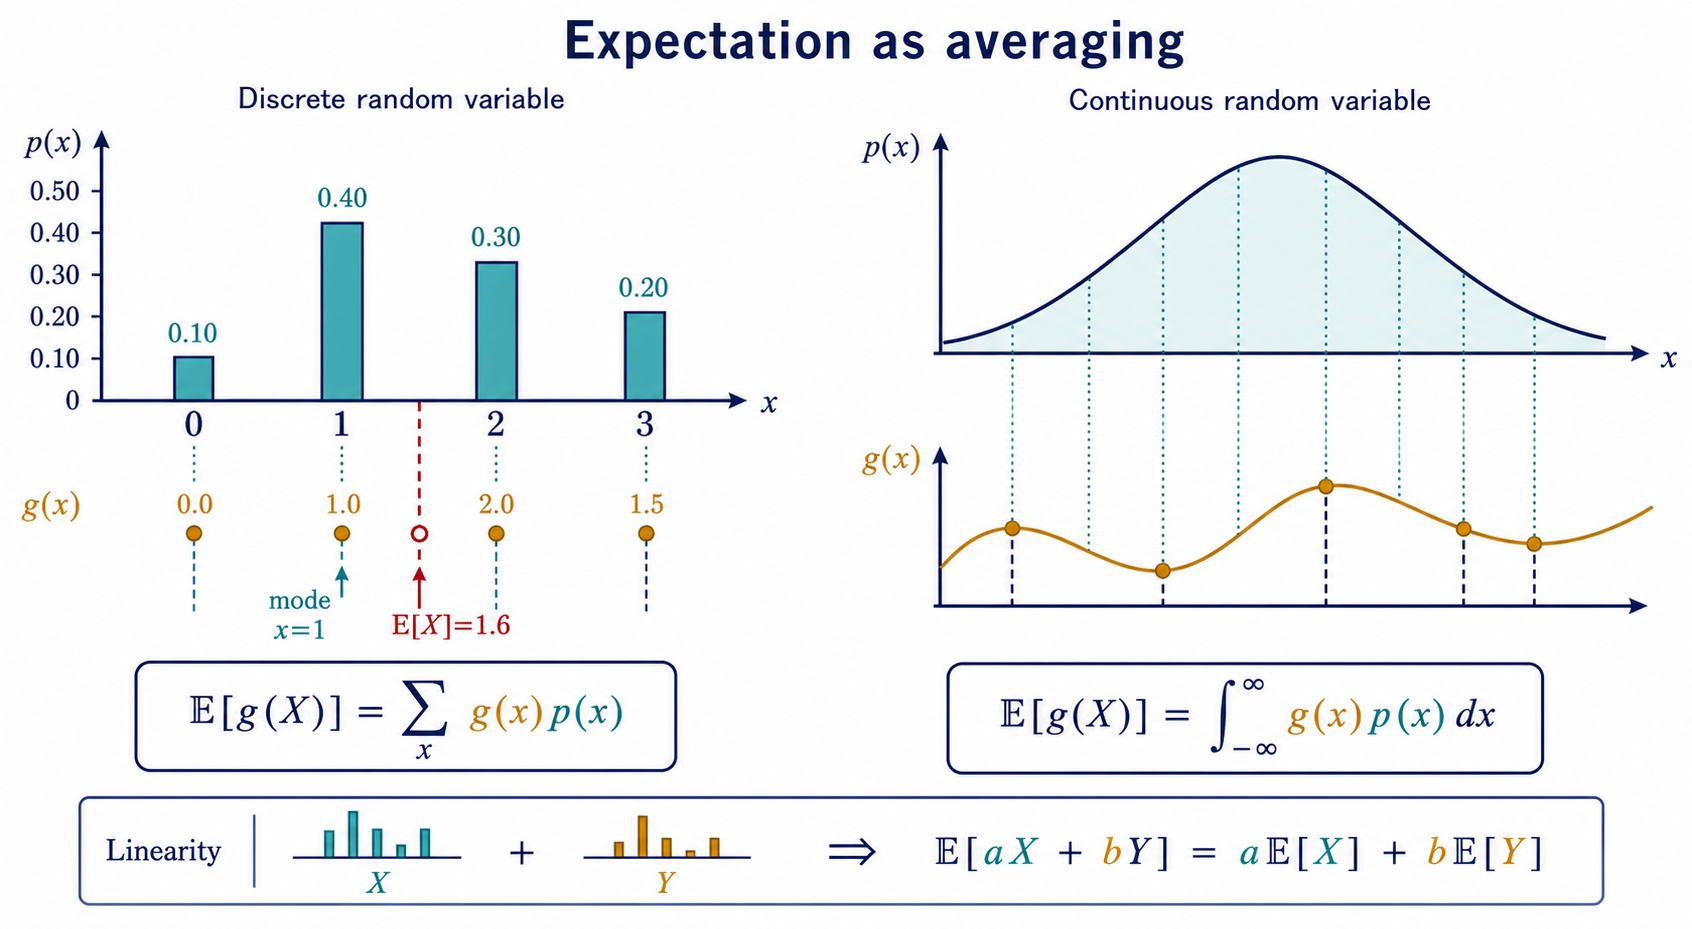
\includegraphics[width=0.98\linewidth]{imagegen-figures/ch15-expectation-averaging.png}
\caption{Expectation is probability-weighted averaging. In the discrete example, the most likely value is the mode \(x=1\), while the balance point is the expectation \(\mathbb{E}[X]=1.6\). For a function of a random variable, \(\mathbb{E}[g(X)]\) is a weighted sum or integral, and linearity says that averaging can pass through addition and scalar multiplication.}
\label{fig:ch15-expectation-averaging}
\end{figure}

\paragraph{Formal setup.}
Let \(X:\Omega\to S\) be a random variable on a probability space \((\Omega,\mathcal{F},P)\). Let \(g:S\to\mathbb{R}\) be a measurable function. The expectation of \(g(X)\) exists when the positive and negative parts of \(g(X)\) are integrable, or more simply in most beginner examples when \(\mathbb{E}[|g(X)|]<\infty\).

If \(X\) is discrete with probability mass function \(p_X(x)=P(X=x)\), then
\[
\boxed{\mathbb{E}[g(X)]=\sum_x g(x)p_X(x).}
\]
If \(X\) is continuous with density \(p_X(x)\), then
\[
\boxed{\mathbb{E}[g(X)]=\int_{-\infty}^{\infty} g(x)p_X(x)\,dx.}
\]
Both formulas are special cases of integration with respect to the distribution \(P_X\):
\[
\mathbb{E}[g(X)] = \int_S g(x)\,dP_X(x).
\]
For \(g(x)=x\), this gives \(\mathbb{E}[X]\). For \(g(x)=(x-\mu)^2\), with \(\mu=\mathbb{E}[X]\), it gives the variance
\[
\operatorname{Var}(X)=\mathbb{E}\!\left[(X-\mathbb{E}[X])^2\right].
\]

\paragraph{Core intuition.}
Figure~\ref{fig:ch15-expectation-averaging} shows expectation as a two-step operation. First, the probability model assigns weights to possible values. Second, the quantity of interest \(g(x)\) is averaged with those weights. The values with larger probability contribute more, but they do not necessarily determine the answer alone. A rare value with a very large \(g(x)\) can strongly affect \(\mathbb{E}[g(X)]\).

In a continuous model, the same picture becomes an integral. The density \(p(x)\) is not itself a probability at a point. Instead, \(g(x)p(x)\,dx\) contributes a small amount of weighted average over a tiny interval. Adding those contributions across the real line gives the expectation.

Common misconceptions are predictable. First, the expected value need not be an outcome. A die roll has expectation \(3.5\), but no face shows \(3.5\). Second, expectation is not the mode. In the discrete example above, the most likely value is \(1\), while the expectation is \(1.6\). Third, expectation can hide risk. A gamble with average payoff \(0\) may still have enormous variance.

This section reuses Chapter 13's random-variable and distribution notation and Chapter 14's distribution catalog. It prepares Chapter 16, where sample averages converge to expectations, and Chapter 17, where risks and likelihood-based objectives are expectations under data-generating distributions.

\paragraph{Main theorem: linearity of expectation.}
If \(X\) and \(Y\) are integrable random variables and \(a,b\in\mathbb{R}\), then
\[
\boxed{\mathbb{E}[aX+bY]=a\mathbb{E}[X]+b\mathbb{E}[Y].}
\]
No independence assumption is required.

\emph{Proof sketch.}
For a finite sample space, expectation is an ordinary weighted sum over outcomes:
\[
\mathbb{E}[aX+bY]
=\sum_{\omega\in\Omega}\bigl(aX(\omega)+bY(\omega)\bigr)P(\{\omega\}).
\]
Distribute the weight \(P(\{\omega\})\) and split the sum:
\[
\sum_{\omega}aX(\omega)P(\{\omega\})
+
\sum_{\omega}bY(\omega)P(\{\omega\}).
\]
Constants can be pulled out:
\[
a\sum_{\omega}X(\omega)P(\{\omega\})
+
b\sum_{\omega}Y(\omega)P(\{\omega\})
=a\mathbb{E}[X]+b\mathbb{E}[Y].
\]
For densities or general integrals, the same mechanism is linearity of integration. Independence is irrelevant because we never factor a joint probability; we only use that averaging is a linear operation.

\paragraph{Worked examples.}
\emph{Small numerical example.} Let \(X\) be the result of a fair die roll. Then
\[
\mathbb{E}[X]
=\frac{1+2+3+4+5+6}{6}
=3.5.
\]
For the squared value,
\[
\mathbb{E}[X^2]
=\frac{1^2+2^2+3^2+4^2+5^2+6^2}{6}
=\frac{91}{6}.
\]
Thus
\[
\operatorname{Var}(X)
=\mathbb{E}[X^2]-(\mathbb{E}[X])^2
=\frac{91}{6}-\frac{49}{4}
=\frac{35}{12}.
\]
The mean \(3.5\) describes the balance point; the variance \(35/12\) describes the spread around it.

\emph{ML/neuroscience example.} Suppose a neuron's spike count \(N\) in a short time window is modeled as Poisson with rate \(\lambda=4\). Chapter 14 introduced the Poisson distribution:
\[
P(N=n)=e^{-\lambda}\frac{\lambda^n}{n!},\qquad n=0,1,2,\ldots.
\]
For a Poisson random variable, \(\mathbb{E}[N]=\lambda\), so the model predicts an average of \(4\) spikes per trial. If an encoder-decoder model pays squared error loss
\[
L=(N-\widehat N)^2,
\]
then \(\mathbb{E}[L]\) is the model's average squared decoding error over repeated trials. The random variable is the trial-to-trial spike count; the expectation is the performance measure averaged over the response distribution.

\paragraph{ML/DL/neuroscience connections.}
In supervised learning, empirical risk is an average over a dataset and population risk is an expectation over the data distribution:
\[
R(f)=\mathbb{E}_{(X,Y)}[\ell(f(X),Y)].
\]
The input-label pair \((X,Y)\) is the random variable, \(\ell(f(X),Y)\) is the loss-valued function, and \(R(f)\) is the expected loss. In deep learning, minibatch gradients approximate expectations of loss gradients. In neuroscience, mean firing rates, average reaction times, expected reward, and average decoding error are all expectations of random variables extracted from trials.

\paragraph{Exercises.}
\begin{enumerate}[label=\textbf{15.1.\arabic*.}, leftmargin=*]
\item \textbf{Mechanical.} A random variable \(X\) has \(P(X=0)=0.2\), \(P(X=2)=0.5\), and \(P(X=5)=0.3\). Compute \(\mathbb{E}[X]\), \(\mathbb{E}[X^2]\), and \(\operatorname{Var}(X)\).
\item \textbf{Proof or derivation.} Use the discrete definition of expectation to prove that \(\mathbb{E}[X+c]=\mathbb{E}[X]+c\) for any constant \(c\).
\item \textbf{Numerical/computational.} A model has losses \(0.1,0.3,0.4,1.2,2.0\) on five equally weighted examples. Compute the empirical expected loss. Then recompute it if the last example has weight \(0.5\) and the other four examples have weight \(0.125\) each.
\item \textbf{Interpretation.} Explain why the expected value of a die roll is \(3.5\) even though no die face is \(3.5\).
\item \textbf{Debug the misconception.} A student says, "The most likely spike count is the expected spike count." Give a distribution where the mode and expectation differ, and explain the difference.
\end{enumerate}

\subsection{15.2 Conditional expectation}

\paragraph{Motivating question.}
How should an average change when we observe partial information such as a stimulus, a measurement, or another random variable?

\paragraph{Beginner setup.}
Conditional expectation is expectation after information is supplied. If \(X\) is an uncertain quantity and \(Y\) is observed information, then \(\mathbb{E}[X\mid Y=y]\) is the average of \(X\) among outcomes for which \(Y=y\).

Consider this joint distribution:
\[
\begin{array}{c|ccc}
 & X=0 & X=1 & X=2\\
\hline
Y=\mathrm{low} & 0.10 & 0.20 & 0.10\\
Y=\mathrm{high} & 0.05 & 0.15 & 0.40
\end{array}
\]
The event \(Y=\mathrm{high}\) has probability \(0.05+0.15+0.40=0.60\). Renormalizing that row gives
\[
P(X=0\mid Y=\mathrm{high})=\frac{0.05}{0.60},\quad
P(X=1\mid Y=\mathrm{high})=\frac{0.15}{0.60},\quad
P(X=2\mid Y=\mathrm{high})=\frac{0.40}{0.60}.
\]
Therefore
\[
\mathbb{E}[X\mid Y=\mathrm{high}]
=0\frac{0.05}{0.60}
+1\frac{0.15}{0.60}
+2\frac{0.40}{0.60}
=\frac{19}{12}\approx 1.58.
\]
For \(Y=\mathrm{low}\), the conditional expectation is \(1\). So \(\mathbb{E}[X\mid Y]\) is not one fixed number; it is a function of the observed value of \(Y\).

Conditional expectation solves a prediction problem. If we have not observed \(Y\), the best single average predictor of \(X\) is often \(\mathbb{E}[X]\). After observing \(Y=y\), the relevant average is \(\mathbb{E}[X\mid Y=y]\). This is the mathematical core of regression, filtering, and many forms of decoding.

What to keep in mind: conditioning is not just selecting a formula with a vertical bar. It changes the probability measure by restricting or updating to the information available. Conditional expectation given a random variable is itself a random variable because it depends on what value of \(Y\) is observed.

\begin{figure}[htbp]
\centering
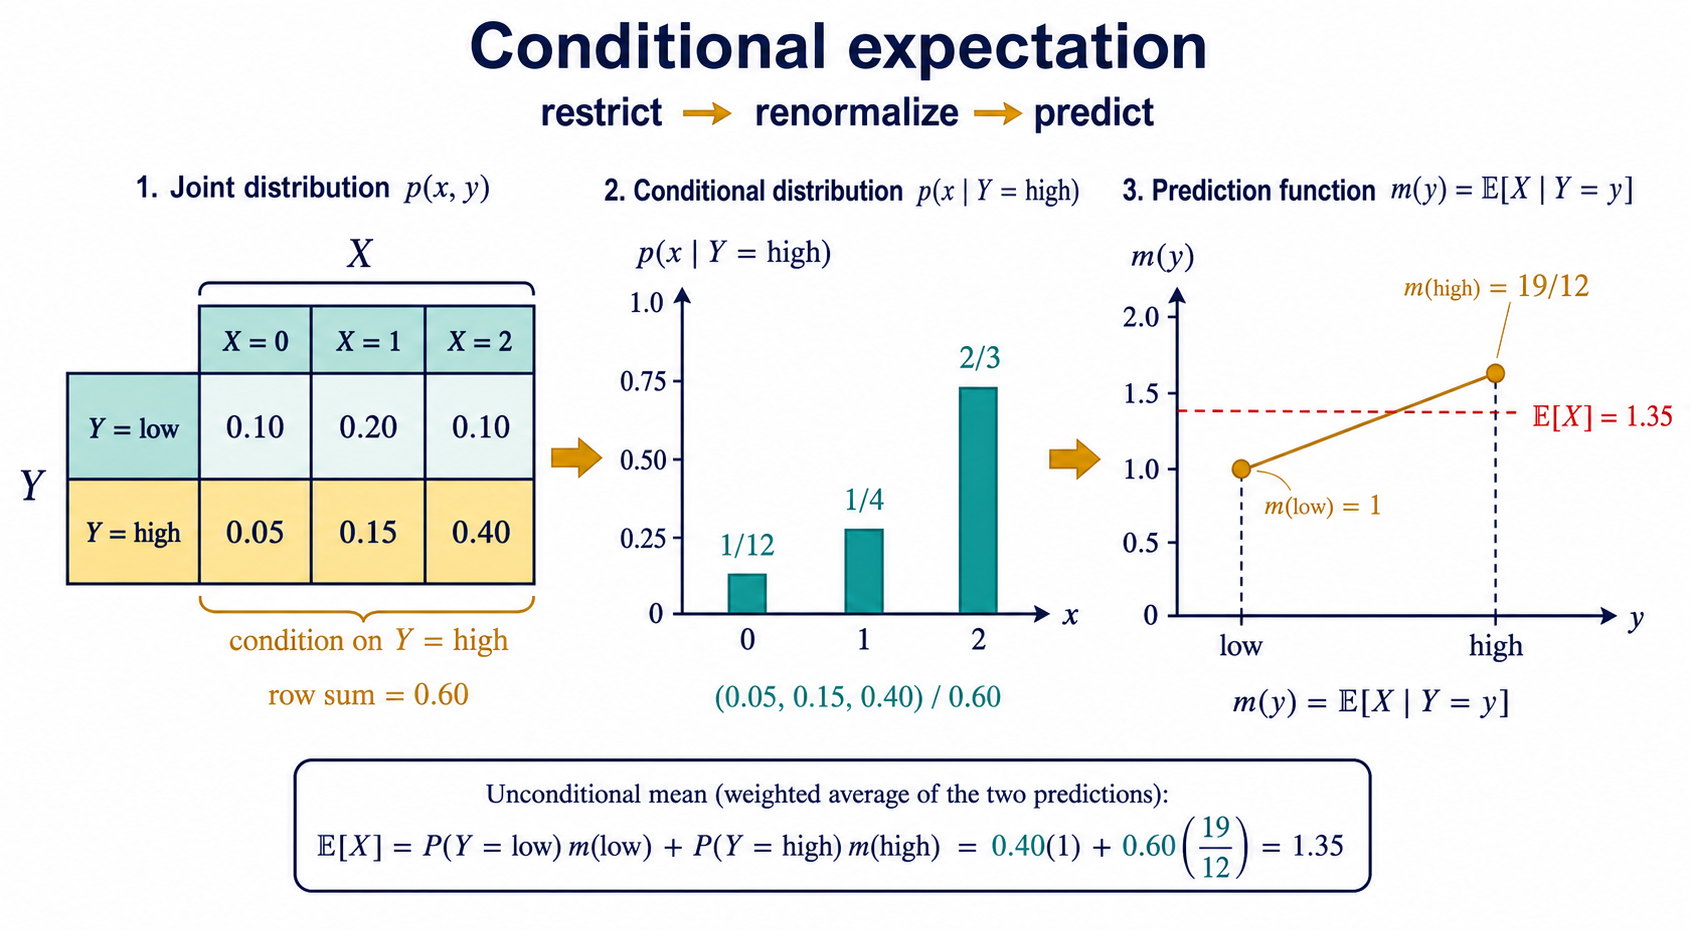
\includegraphics[width=0.98\linewidth]{imagegen-figures/ch15-conditional-expectation.png}
\caption{Conditional expectation begins with a joint distribution. Conditioning on \(Y=\mathrm{high}\) selects and renormalizes one row, producing \(p(x\mid Y=\mathrm{high})\). The conditional expectation function \(m(y)=\mathbb{E}[X\mid Y=y]\) is the prediction of \(X\) based only on the observed information \(Y=y\).}
\label{fig:ch15-conditional-expectation}
\end{figure}

\paragraph{Formal setup.}
For an event \(B\) with \(P(B)>0\), the conditional expectation of an integrable random variable \(X\) given \(B\) is
\[
\mathbb{E}[X\mid B]
=\frac{\mathbb{E}[X\mathbf{1}_B]}{P(B)}.
\]
For a discrete random variable \(Y\), with \(P(Y=y)>0\),
\[
\boxed{\mathbb{E}[X\mid Y=y]=\sum_x x\,p_{X\mid Y}(x\mid y).}
\]
For continuous \(X\), replace the sum with an integral:
\[
\mathbb{E}[X\mid Y=y]
=\int x\,p_{X\mid Y}(x\mid y)\,dx.
\]

The conditional expectation given \(Y\), written \(\mathbb{E}[X\mid Y]\), is the random variable
\[
m(Y),\qquad m(y)=\mathbb{E}[X\mid Y=y],
\]
in the discrete setting. In the general measure-theoretic setting, \(\mathbb{E}[X\mid Y]\) means \(\mathbb{E}[X\mid \sigma(Y)]\), the best prediction of \(X\) using only events determined by \(Y\). We will use the concrete \(m(Y)\) viewpoint in this chapter.

\paragraph{Core intuition.}
Figure~\ref{fig:ch15-conditional-expectation} shows three views. The joint table contains all probability mass for the pair \((X,Y)\). Observing \(Y=\mathrm{high}\) selects one slice. Dividing by the slice probability renormalizes it into a conditional distribution. Averaging \(X\) under that conditional distribution gives one value of the prediction function \(m(y)\).

The phrase "using only information in \(Y\)" is important. If \(Y\) is a stimulus category, \(\mathbb{E}[X\mid Y]\) predicts a response from the stimulus category but ignores trial-specific noise not contained in \(Y\). If \(Y\) is a partial neural recording, \(\mathbb{E}[X\mid Y]\) predicts the unobserved quantity from that recording.

Common misconceptions: First, \(\mathbb{E}[X\mid Y]\) is not usually equal to \(\mathbb{E}[X]\). Equality means observing \(Y\) does not change the average of \(X\), which is a special situation. Second, \(\mathbb{E}[X\mid Y]\) is not the same object as \(\mathbb{E}[Y\mid X]\). They answer different prediction questions. Third, conditioning on a value with probability zero needs density or regular-conditional-probability machinery; beginner formulas such as \(P(A\mid B)=P(A\cap B)/P(B)\) require \(P(B)>0\).

This section connects backward to Chapter 13's conditional distributions and forward to filtering, graphical models, predictive coding, and regression. In a Kalman filter, for example, the current posterior mean is a conditional expectation of the hidden state given observations so far.

\paragraph{Main theorem: conditional expectation is the best mean-square prediction from \(Y\).}
In the finite discrete setting, let \(X\) be square-integrable and let \(Y\) take finitely many values. Among all functions \(h(Y)\), the function
\[
m(Y)=\mathbb{E}[X\mid Y]
\]
minimizes
\[
\mathbb{E}\!\left[(X-h(Y))^2\right].
\]

\emph{Proof sketch.}
Group the mean-square error by the value of \(Y\):
\[
\mathbb{E}\!\left[(X-h(Y))^2\right]
=\sum_y P(Y=y)\,
\mathbb{E}\!\left[(X-h(y))^2\mid Y=y\right].
\]
For a fixed \(y\), the only adjustable number is \(h(y)\). Let \(c=h(y)\). Expand the conditional squared error:
\[
\mathbb{E}\!\left[(X-c)^2\mid Y=y\right]
=\mathbb{E}\!\left[(X-m(y)+m(y)-c)^2\mid Y=y\right].
\]
The cross term vanishes because
\[
\mathbb{E}[X-m(y)\mid Y=y]=0.
\]
So
\[
\mathbb{E}\!\left[(X-c)^2\mid Y=y\right]
=\mathbb{E}\!\left[(X-m(y))^2\mid Y=y\right]+(m(y)-c)^2.
\]
This is minimized when \(c=m(y)\). Since each \(y\)-slice is minimized by \(h(y)=m(y)\), the whole weighted sum is minimized by \(h(Y)=\mathbb{E}[X\mid Y]\). The mechanism is projection: conditional expectation is the closest prediction to \(X\) among all functions of the observed information.

\paragraph{Worked examples.}
\emph{Small numerical example.} Using the table above,
\[
P(Y=\mathrm{low})=0.40,\qquad P(Y=\mathrm{high})=0.60.
\]
The conditional expectations are
\[
\mathbb{E}[X\mid Y=\mathrm{low}]
=0\frac{0.10}{0.40}+1\frac{0.20}{0.40}+2\frac{0.10}{0.40}
=1,
\]
and
\[
\mathbb{E}[X\mid Y=\mathrm{high}]
=\frac{19}{12}.
\]
The conditional expectation random variable is therefore
\[
\mathbb{E}[X\mid Y]
=
\begin{cases}
1, & Y=\mathrm{low},\\
19/12, & Y=\mathrm{high}.
\end{cases}
\]
Its average recovers the unconditional mean:
\[
\mathbb{E}[\mathbb{E}[X\mid Y]]
=0.40(1)+0.60\left(\frac{19}{12}\right)
=1.35
=\mathbb{E}[X].
\]
This identity is called the tower property or law of total expectation.

\emph{ML/neuroscience example.} Let \(X\) be a hand position to decode and let \(Y\) be the spike counts from a motor-cortex population in a short window. A decoder that outputs
\[
\widehat X(Y)=\mathbb{E}[X\mid Y]
\]
is the best mean-square predictor among all decoders that use only those spike counts. The mathematical mapping is explicit: \(X\) is the latent movement variable, \(Y\) is the observed neural response vector, and \(\mathbb{E}[X\mid Y]\) is the decoding function. In practice the conditional expectation must be estimated from a probabilistic model or data.

\paragraph{ML/DL/neuroscience connections.}
Regression functions are conditional expectations under squared loss:
\[
f^*(x)=\mathbb{E}[Y\mid X=x].
\]
Filtering algorithms compute conditional expectations of hidden states given observations. In predictive coding, predictions can be interpreted as conditional expectations of sensory input or latent causes under an internal model. In neural decoding, the same object appears when estimating a stimulus, movement, or decision variable from observed neural activity.

\paragraph{Exercises.}
\begin{enumerate}[label=\textbf{15.2.\arabic*.}, leftmargin=*]
\item \textbf{Mechanical.} In the joint table from this section, compute \(P(X=2\mid Y=\mathrm{high})\), \(P(X=2\mid Y=\mathrm{low})\), and \(\mathbb{E}[X\mid Y=\mathrm{low}]\).
\item \textbf{Proof or derivation.} Prove the tower property \(\mathbb{E}[\mathbb{E}[X\mid Y]]=\mathbb{E}[X]\) for finite discrete \(X\) and \(Y\) by expanding both sides as sums over \(x\) and \(y\).
\item \textbf{Numerical/computational.} A decoder predicts movement speed from a neural feature \(Y\in\{0,1\}\). From data, the speeds for \(Y=0\) are \(1.1,0.9,1.0\), and the speeds for \(Y=1\) are \(2.0,2.2,1.8,2.4\). Estimate \(\mathbb{E}[X\mid Y=0]\) and \(\mathbb{E}[X\mid Y=1]\).
\item \textbf{Interpretation.} Explain why \(\mathbb{E}[X\mid Y]\) should be treated as a random variable before \(Y\) is observed and as a number after a value \(Y=y\) is observed.
\item \textbf{Debug the misconception.} A student says, "If I know \(\mathbb{E}[X]\), then conditioning on \(Y\) cannot change the average." Use the table in this section to show why this is false.
\end{enumerate}

\subsection{15.3 Bayes' theorem}

\paragraph{Motivating question.}
If a model tells us how likely data are under each hypothesis, how do we reverse the direction and compute how likely each hypothesis is after seeing the data?

\paragraph{Beginner setup.}
Bayes' theorem is a rule for updating beliefs about hypotheses after observing evidence. Suppose \(\Theta\) is an uncertain hypothesis and \(X\) is observed data. Before seeing \(X=x\), uncertainty about \(\Theta\) is described by a prior \(p(\theta)\). The model for data under a hypothesis is the likelihood \(p(x\mid \theta)\). After observing \(x\), the posterior distribution is
\[
p(\theta\mid x).
\]
Bayes' theorem says
\[
\text{posterior}
=
\frac{\text{likelihood}\times\text{prior}}{\text{evidence}}.
\]

The smallest useful example has two hypotheses. A rare condition has prior probability \(P(\Theta=1)=0.01\). A test is positive with probability \(0.99\) if the condition is present and \(0.05\) if absent. If \(X=+\) denotes a positive test, then
\[
P(\Theta=1\mid X=+)
=\frac{P(X=+\mid \Theta=1)P(\Theta=1)}
{P(X=+\mid \Theta=1)P(\Theta=1)+P(X=+\mid \Theta=0)P(\Theta=0)}.
\]
Numerically,
\[
P(\Theta=1\mid X=+)
=\frac{0.99(0.01)}{0.99(0.01)+0.05(0.99)}
=\frac{0.0099}{0.0594}
=\frac16.
\]
Even a positive test leaves posterior probability far below \(0.99\) because the base rate is low.

Bayes solves the inverse problem of inference. Forward models often describe how causes generate observations. Science and learning often need the reverse: infer causes from observations.

What to keep in mind: Bayes' theorem does not say \(P(\Theta\mid X)=P(X\mid \Theta)\). The likelihood is a function of the hypothesis for fixed data; the posterior is a probability distribution over hypotheses after normalization.

\begin{figure}[htbp]
\centering
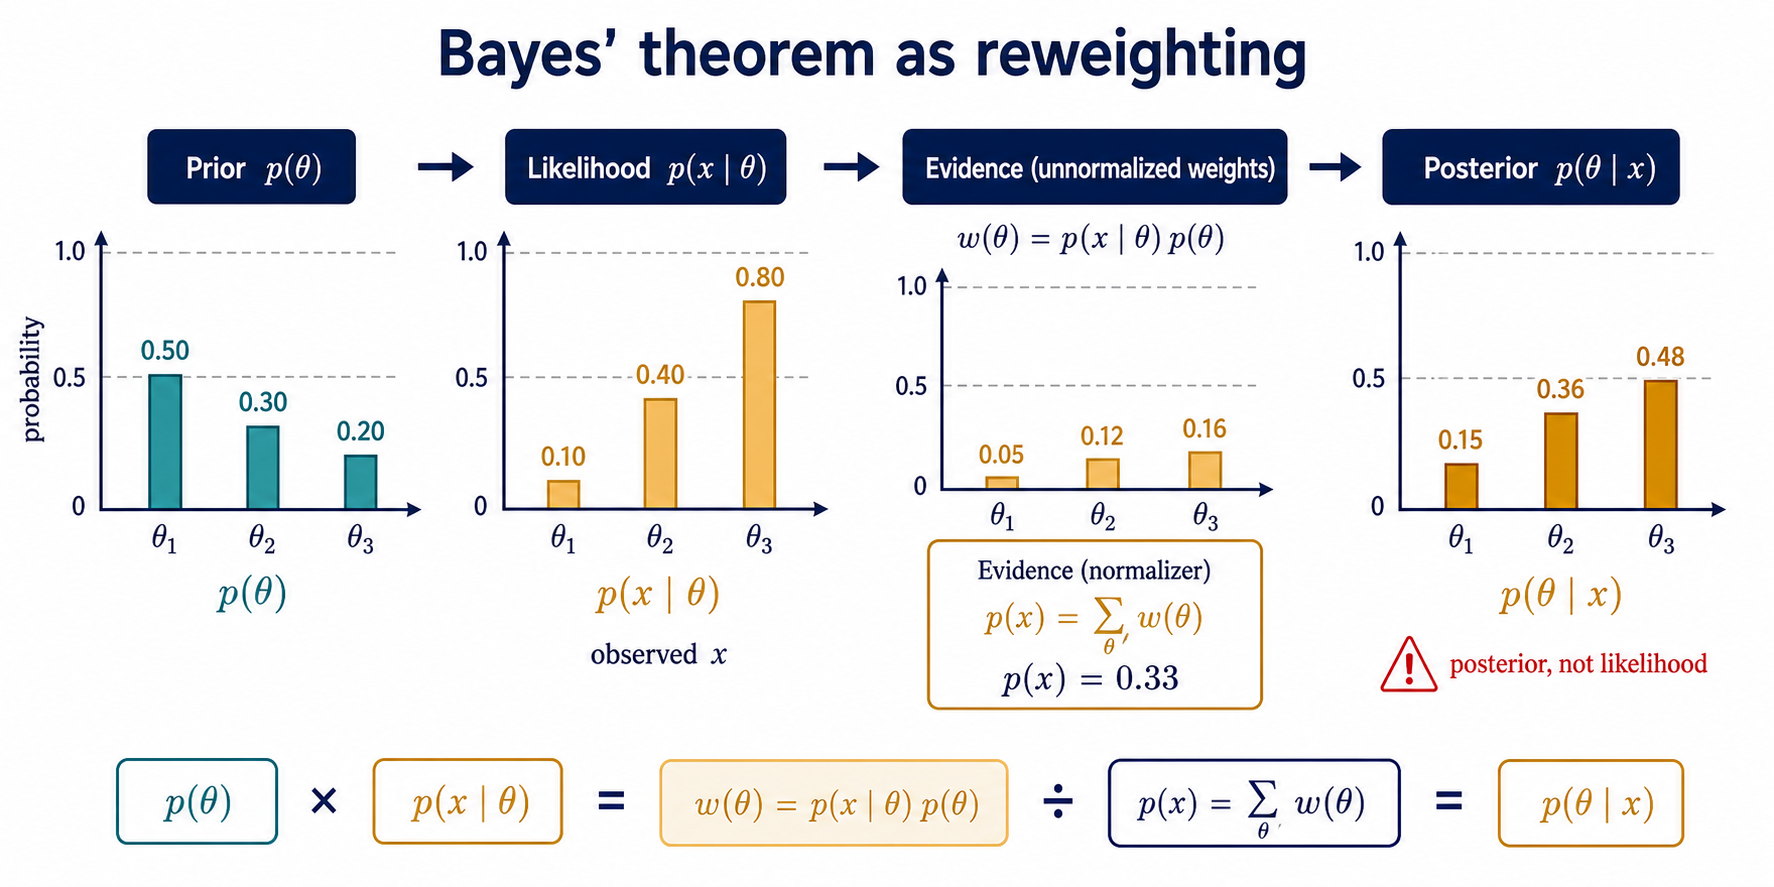
\includegraphics[width=0.98\linewidth]{imagegen-figures/ch15-bayes-reweighting.png}
\caption{Bayes' theorem reweights hypotheses. The prior \(p(\theta)\) is multiplied by the likelihood \(p(x\mid \theta)\) for the observed data \(x\), then normalized by the evidence \(p(x)=\sum_\theta p(x\mid \theta)p(\theta)\) to produce the posterior \(p(\theta\mid x)\).}
\label{fig:ch15-bayes-reweighting}
\end{figure}

\paragraph{Formal setup.}
For events \(A\) and \(B\) with \(P(A)>0\) and \(P(B)>0\),
\[
\boxed{P(A\mid B)=\frac{P(B\mid A)P(A)}{P(B)}.}
\]
The denominator can always be expanded by partitioning over \(A\) and \(A^c\):
\[
P(B)=P(B\cap A)+P(B\cap A^c).
\]
If \(0<P(A)<1\), this becomes the conditional-probability form
\[
P(B)=P(B\mid A)P(A)+P(B\mid A^c)P(A^c).
\]

For a discrete hypothesis \(\Theta\in\mathcal{T}\) and observed data \(X=x\), assume the evidence
\[
p(x)=\sum_{\theta'\in\mathcal{T}}p(x\mid \theta')p(\theta')
\]
is positive. Then Bayes' theorem becomes
\[
\boxed{
p(\theta\mid x)
=
\frac{p(x\mid \theta)p(\theta)}
{\sum_{\theta'\in\mathcal{T}}p(x\mid \theta')p(\theta')}
}.
\]
For a continuous parameter \(\theta\), assume the evidence
\[
p(x)=\int p(x\mid \theta')p(\theta')\,d\theta'
\]
is positive and finite. Then the denominator is an integral:
\[
p(\theta\mid x)
=
\frac{p(x\mid \theta)p(\theta)}
{\int p(x\mid \theta')p(\theta')\,d\theta'}.
\]
The denominator is called the evidence, marginal likelihood, or normalizing constant.

If data \(X_1,\ldots,X_n\) are conditionally independent given \(\Theta\), then the likelihood factorizes:
\[
p(x_1,\ldots,x_n\mid \theta)
=\prod_{i=1}^n p(x_i\mid \theta).
\]
This conditional independence assumption is what lets many Bayesian models combine repeated measurements cleanly.

\paragraph{Core intuition.}
Figure~\ref{fig:ch15-bayes-reweighting} presents Bayes' theorem as reweighting. Start with prior weights over hypotheses. The observed data assign each hypothesis a likelihood score. Multiplying prior by likelihood gives unnormalized posterior weights. Dividing by the evidence rescales those weights to sum or integrate to \(1\).

The evidence is not an optional detail. Without it, \(p(x\mid \theta)p(\theta)\) has the right relative weights but is not yet a probability distribution over \(\theta\). In model comparison, the evidence also measures how well a whole model predicts the observed data after averaging over its parameters.

Common misconceptions: First, do not reverse a conditional without the prior and evidence. \(P(\text{positive}\mid \text{condition})\) and \(P(\text{condition}\mid \text{positive})\) answer different questions. Second, the likelihood is not a probability distribution over \(\theta\) until it is multiplied by a prior and normalized. Third, independence and conditional independence are different. Two observations may be dependent marginally but independent once the hidden cause \(\Theta\) is known.

This section connects Chapter 14's likelihoods to Chapter 17's inference. It also prepares graphical models and predictive coding, where conditional independence assumptions determine which likelihood factors appear in a posterior update.

\paragraph{Main theorem: Bayes' theorem from two factorizations of a joint probability.}
If \(P(A)>0\) and \(P(B)>0\), then
\[
P(A\mid B)=\frac{P(B\mid A)P(A)}{P(B)}.
\]

\emph{Proof sketch.}
The joint event \(A\cap B\) can be factored in two ways:
\[
P(A\cap B)=P(A\mid B)P(B),
\]
and
\[
P(A\cap B)=P(B\mid A)P(A).
\]
Both equations describe the same overlap. Setting the right sides equal gives
\[
P(A\mid B)P(B)=P(B\mid A)P(A).
\]
Because \(P(B)>0\), divide by \(P(B)\):
\[
P(A\mid B)=\frac{P(B\mid A)P(A)}{P(B)}.
\]
For a hypothesis variable \(\Theta\), the same proof uses the joint density or mass \(p(x,\theta)\) and the two factorizations
\[
p(x,\theta)=p(\theta\mid x)p(x)=p(x\mid \theta)p(\theta).
\]

\paragraph{Worked examples.}
\emph{Small numerical example.} In the diagnostic example above,
\[
P(\Theta=1)=0.01,\quad
P(X=+\mid \Theta=1)=0.99,\quad
P(X=+\mid \Theta=0)=0.05.
\]
The evidence is
\[
P(X=+)=0.99(0.01)+0.05(0.99)=0.0594.
\]
The posterior is
\[
P(\Theta=1\mid X=+)=0.0099/0.0594=1/6.
\]
The base rate prevents the positive test from implying near certainty.

\emph{ML/neuroscience example.} A simple neural decoder has two possible stimuli, \(S\in\{\mathrm{left},\mathrm{right}\}\). Suppose the prior is uniform. A neuron emits \(N\) spikes in a window, with
\[
N\mid S=\mathrm{left}\sim\operatorname{Poisson}(2),
\qquad
N\mid S=\mathrm{right}\sim\operatorname{Poisson}(6).
\]
If \(N=5\), then
\[
P(S=\mathrm{right}\mid N=5)
=
\frac{P(N=5\mid S=\mathrm{right})P(S=\mathrm{right})}
{P(N=5\mid S=\mathrm{left})P(S=\mathrm{left})
+P(N=5\mid S=\mathrm{right})P(S=\mathrm{right})}.
\]
The equal priors cancel, so
\[
P(S=\mathrm{right}\mid N=5)
=
\frac{e^{-6}6^5/5!}{e^{-2}2^5/5!+e^{-6}6^5/5!}
\approx 0.80.
\]
The objects map directly: \(S\) is the stimulus hypothesis, \(N\) is the observed spike count, the Poisson distributions are likelihoods, and the posterior is the decoded stimulus belief.

\paragraph{ML/DL/neuroscience connections.}
Bayesian inference appears whenever a model combines a prior with a likelihood. In Bayesian neural decoding, the posterior \(p(s\mid r)\) represents a belief over stimuli \(s\) after observing response \(r\). In latent-variable models, \(p(z\mid x)\) is the posterior over latent causes after observing data. In variational inference, an approximate posterior \(q(z\mid x)\) is trained to resemble the true posterior. In graphical models, conditional independence assumptions make the likelihood factor into local pieces.

\paragraph{Exercises.}
\begin{enumerate}[label=\textbf{15.3.\arabic*.}, leftmargin=*]
\item \textbf{Mechanical.} A disease has prior \(P(D)=0.02\). A test has \(P(+\mid D)=0.90\) and \(P(+\mid D^c)=0.10\). Compute \(P(D\mid +)\).
\item \textbf{Proof or derivation.} Starting from \(p(x,\theta)=p(x\mid\theta)p(\theta)=p(\theta\mid x)p(x)\), derive the discrete Bayes formula with the evidence written as a sum over \(\theta'\).
\item \textbf{Numerical/computational.} Three stimuli have priors \(0.5,0.3,0.2\). For an observed response \(r\), their likelihoods are \(0.1,0.4,0.8\). Compute the normalized posterior over the three stimuli.
\item \textbf{Interpretation.} In the diagnostic example, why is \(P(\Theta=1\mid X=+)\) much smaller than \(P(X=+\mid \Theta=1)\)?
\item \textbf{Debug the misconception.} A student says, "The likelihood \(p(x\mid\theta)\) already sums to one over \(\theta\)." Explain why this is not generally true and what normalization Bayes' theorem performs.
\end{enumerate}

\subsection{15.4 Bayesian decision theory}

\paragraph{Motivating question.}
Once we have a posterior distribution, how do we choose an action when different mistakes have different costs?

\paragraph{Beginner setup.}
Bayesian decision theory adds actions and losses to Bayesian inference. A posterior distribution says what states are plausible after observing data. A loss function says how bad each action is under each state. The decision rule chooses the action with smallest posterior expected loss.

For a two-state example, suppose \(\Theta=1\) means a stimulus is present and \(\Theta=0\) means absent. After observing data \(x\), assume
\[
P(\Theta=1\mid x)=0.30,\qquad P(\Theta=0\mid x)=0.70.
\]
There are two actions: report present or report absent. A false alarm costs \(1\), but a miss costs \(5\). The posterior risk of reporting present is
\[
R(\mathrm{present}\mid x)=1\cdot P(\Theta=0\mid x)=0.70.
\]
The posterior risk of reporting absent is
\[
R(\mathrm{absent}\mid x)=5\cdot P(\Theta=1\mid x)=1.50.
\]
Even though \(\Theta=1\) is not the more likely state, the lower-risk action is to report present because misses are more costly.

Decision theory solves the final step from belief to action. Bayes' theorem gives a posterior, but the posterior alone does not say what to do. The right action depends on the loss or utility attached to each possible mistake.

What to keep in mind: the most probable state and the best action can differ. MAP estimation chooses the most probable state under 0-1 loss. Other losses produce other decisions, such as posterior means under squared-error loss or conservative thresholds under asymmetric costs.

\begin{figure}[htbp]
\centering
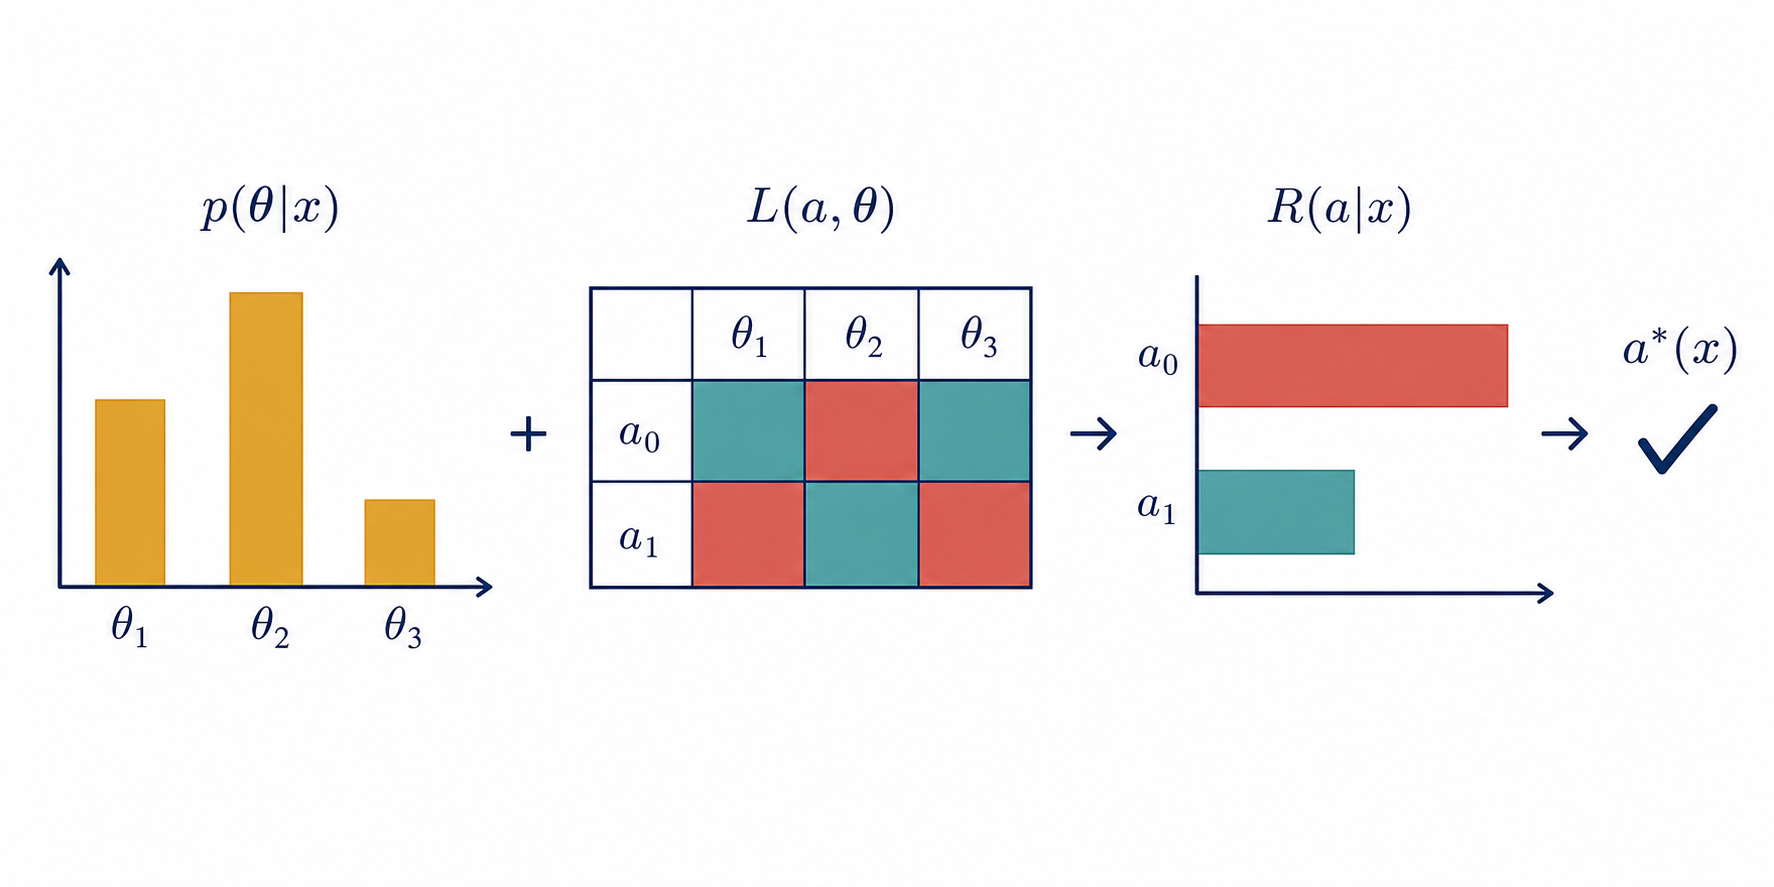
\includegraphics[width=0.95\linewidth]{imagegen-figures/ch15-bayesian-decision-risk.png}
\caption{Bayesian decision theory combines posterior beliefs with a loss function. The posterior \(p(\theta\mid x)\) describes uncertainty over states, the loss matrix \(L(a,\theta)\) assigns costs to action-state pairs, and posterior risk \(R(a\mid x)\) averages those costs. The Bayes action \(a^*(x)\) is the action with smallest posterior risk.}
\label{fig:ch15-bayesian-decision-risk}
\end{figure}

\paragraph{Formal setup.}
Let \(\Theta\) be an unknown state or parameter taking values in a state space \(\mathcal{T}\), let \(X=x\) be the observed data, and let \(\mathcal{A}\) be a set of possible actions. A loss function
\[
L:\mathcal{A}\times\mathcal{T}\to\mathbb{R}
\]
assigns cost \(L(a,\theta)\) to taking action \(a\) when the true state is \(\theta\). The posterior risk of action \(a\) after observing \(x\) is
\[
\boxed{
R(a\mid x)
=\mathbb{E}[L(a,\Theta)\mid X=x].
}
\]
For discrete \(\Theta\),
\[
R(a\mid x)=\sum_{\theta\in\mathcal{T}}L(a,\theta)p(\theta\mid x).
\]
The Bayes action is
\[
\boxed{
a^*(x)\in\operatorname*{arg\,min}_{a\in\mathcal{A}} R(a\mid x).
}
\]
If utilities \(U(a,\theta)\) are used instead of losses, the equivalent rule is to maximize posterior expected utility.

\paragraph{Core intuition.}
Figure~\ref{fig:ch15-bayesian-decision-risk} shows the computation. The posterior gives weights over possible states. The loss matrix gives the cost of each action in each state. Multiplying loss by posterior probability and summing over states gives one risk number per action. The smallest number wins.

This is expectation again, but now the quantity being averaged is a loss. The posterior distribution supplies the weights because the decision is made after observing data. A decision before seeing data would average over the prior predictive distribution instead.

Common misconceptions: First, "Bayesian" does not mean "always choose the MAP state." MAP is the Bayes action only for symmetric 0-1 loss when actions are state guesses. Second, a low posterior probability can still matter when its associated loss is large. Third, the loss function is not a technical afterthought; it encodes the scientific or practical stakes of mistakes.

This section connects to Chapter 17's risk, estimation, testing, confidence, and model selection. It also points to later neural decision-making chapters, where behavior is modeled as accumulation of evidence followed by an action chosen under reward and cost constraints.

\paragraph{Main theorem: MAP and posterior mean as Bayes actions for common losses.}
Suppose the action \(a\) is a point estimate of \(\Theta\).

For discrete \(\Theta\), under 0-1 loss
\[
L(a,\theta)=
\begin{cases}
0, & a=\theta,\\
1, & a\neq \theta,
\end{cases}
\]
any posterior mode
\[
a^*(x)\in\operatorname*{arg\,max}_{\theta}p(\theta\mid x)
\]
is a Bayes action.

For real-valued \(\Theta\), under squared-error loss \(L(a,\theta)=(a-\theta)^2\), the Bayes action is the posterior mean
\[
a^*(x)=\mathbb{E}[\Theta\mid X=x].
\]

\emph{Proof sketch.}
Under 0-1 loss, the posterior risk of choosing action \(a\) is
\[
R(a\mid x)
=\sum_{\theta\neq a}p(\theta\mid x)
=1-p(\Theta=a\mid X=x).
\]
Minimizing \(1-p(\Theta=a\mid X=x)\) is the same as maximizing \(p(\Theta=a\mid X=x)\), so the Bayes action is a MAP choice.

Under squared-error loss, let \(m=\mathbb{E}[\Theta\mid X=x]\). The posterior risk is
\[
R(a\mid x)=\mathbb{E}[(a-\Theta)^2\mid X=x].
\]
Write \(a-\Theta=(a-m)+(m-\Theta)\). Expanding and conditioning on \(X=x\),
\[
R(a\mid x)
=(a-m)^2
+2(a-m)\mathbb{E}[m-\Theta\mid X=x]
+\mathbb{E}[(m-\Theta)^2\mid X=x].
\]
The middle term is zero because \(m=\mathbb{E}[\Theta\mid X=x]\). The last term does not depend on \(a\). Therefore the risk is minimized when \((a-m)^2\) is minimized, namely at \(a=m\).

\paragraph{Worked examples.}
\emph{Small numerical example.} In the asymmetric-cost example,
\[
P(\Theta=1\mid x)=0.30,\qquad P(\Theta=0\mid x)=0.70.
\]
Let action \(a=1\) mean report present and \(a=0\) mean report absent. The loss table is
\[
\begin{array}{c|cc}
& \Theta=0 & \Theta=1\\
\hline
a=0 & 0 & 5\\
a=1 & 1 & 0
\end{array}
\]
Thus
\[
R(0\mid x)=0(0.70)+5(0.30)=1.50,
\]
while
\[
R(1\mid x)=1(0.70)+0(0.30)=0.70.
\]
The Bayes action is \(a^*(x)=1\), even though the MAP state is \(\Theta=0\). Loss changes the decision.

\emph{ML/neuroscience example.} In a brain-computer interface, \(\Theta\) may be the user's intended command and \(X\) the neural recording. The posterior \(p(\theta\mid x)\) is the decoder's belief over commands. The action \(a\) is the command sent to a device. A wrong command that moves a cursor slightly may have low loss, while a wrong command that selects an irreversible option may have high loss. The Bayes action minimizes
\[
R(a\mid x)=\sum_{\theta}L(a,\theta)p(\theta\mid x),
\]
so the decoder can choose a safer action even when it is not simply the most probable command.

\paragraph{ML/DL/neuroscience connections.}
Classification with cross-entropy often trains models to approximate posterior class probabilities; deployment still needs a decision threshold or action rule. Medical AI, autonomous systems, and neural prosthetics usually have asymmetric costs, so a calibrated posterior is only the input to a decision problem. In neuroscience, perceptual decisions can be modeled as choosing an action that trades off posterior belief, reward, time cost, and error penalty. Predictive coding and active inference extend this logic by treating action selection as minimizing expected future cost or surprise under a generative model.

\paragraph{Exercises.}
\begin{enumerate}[label=\textbf{15.4.\arabic*.}, leftmargin=*]
\item \textbf{Mechanical.} A posterior gives \(P(\Theta=1\mid x)=0.4\) and \(P(\Theta=0\mid x)=0.6\). False alarm loss is \(2\), miss loss is \(5\), and correct decisions have loss \(0\). Compute the posterior risk of reporting \(1\) and of reporting \(0\). Which action is Bayes optimal?
\item \textbf{Proof or derivation.} Derive the MAP rule from 0-1 loss by writing the posterior risk \(R(a\mid x)\) and simplifying it.
\item \textbf{Numerical/computational.} Three actions have posterior risks \(0.24,0.19,0.31\) under one observation and \(0.12,0.14,0.11\) under another observation. Choose the Bayes action in each case. Then describe how the answer would change if these numbers were utilities rather than losses.
\item \textbf{Interpretation.} Why can the Bayes action differ from the most probable state when losses are asymmetric?
\item \textbf{Debug the misconception.} A student says, "After computing the posterior, decision theory is automatic: pick the largest posterior probability." State the loss assumption under which this is correct and give one situation where it is not.
\end{enumerate}

\paragraph{Closing bridge.}
This chapter turned probability distributions into prediction and action. Expectation is the averaging operator; conditional expectation is averaging after information; Bayes' theorem updates hypotheses by likelihood-weighted normalization; Bayesian decision theory chooses actions by posterior expected loss. Chapter 16 will ask when empirical averages reliably approximate expectations and why high-dimensional random objects concentrate. Chapter 17 will use the same expectation, conditioning, likelihood, posterior, and risk language to build statistical inference and model selection. Chapter 18 will measure uncertainty and distinguishability by taking expectations of logarithmic probability ratios.

\clearpage
